We now revisit the transient heat equation, this time with sources/sinks for 2D problems.
In the absence of advective heat transport, the heat equation is 
\begin{equation}
\rho C_p \frac{\partial T}{\partial t} =
\vec\nabla \cdot k \vec\nabla T + Q 
\end{equation}
which simply writes as follows when Cartesian coordinates are used:
\begin{equation}
\rho C_p \frac{\partial T}{\partial t} = 
\frac{\partial }{\partial x} \left(  k  \frac{\partial T}{\partial x} \right)+
\frac{\partial }{\partial y} \left(  k  \frac{\partial T}{\partial y} \right)+ Q
\end{equation}
where $Q$ is the radiogenic heat production.

If the heat conductivity is constant, it writes:
\begin{equation}
\frac{\partial T}{\partial t} =
\kappa \left(  \frac{\partial^2 T}{\partial x^2} + \frac{\partial^2 T}{\partial y^2} \right)+
\frac{Q}{\rho C_p}
\end{equation}
In order to solve this equation over the Cartesian domain of size $L_x \times L_y$
we need to generate a mesh as shown hereunder:

%-/-/-/-/-/-/-/-/-/-/-/-/-/-/-/
\begin{minipage}[t]{\textwidth}
\begin{center}


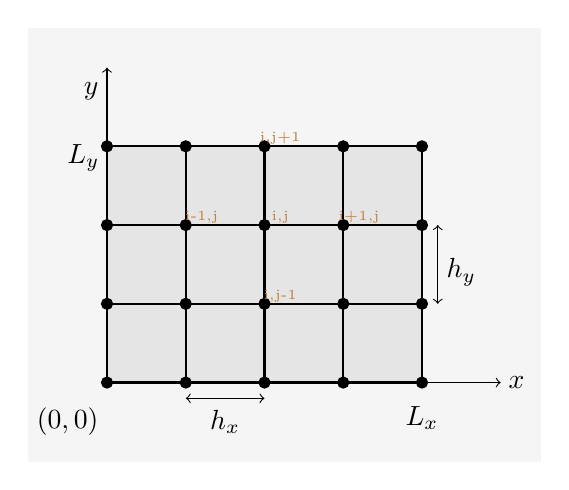
\begin{tikzpicture}
\draw[fill=gray!8,gray!8](0,0) rectangle (6.5,5.5);
%\draw[step=0.5cm,gray,very thin] (0,0) grid (8,5); %background grid


\draw[fill=gray!20,gray!20](1,1) rectangle (5,4);
\draw[thick] (1,1) -- (5,1) -- (5,4) -- (1,4) -- cycle;  

\draw[thick] (1,2) -- (5,2) ; 
\draw[thick] (1,3) -- (5,3) ; 
\draw[thick] (2,1) -- (2,4) ; 
\draw[thick] (3,1) -- (3,4) ; 
\draw[thick] (4,1) -- (4,4) ; 

\draw[black,fill=black] (1,1)  circle (2pt);
\draw[black,fill=black] (2,1)  circle (2pt);
\draw[black,fill=black] (3,1)  circle (2pt);
\draw[black,fill=black] (4,1)  circle (2pt);
\draw[black,fill=black] (5,1)  circle (2pt);
\draw[black,fill=black] (1,2)  circle (2pt);
\draw[black,fill=black] (2,2)  circle (2pt);
\draw[black,fill=black] (3,2)  circle (2pt);
\draw[black,fill=black] (4,2)  circle (2pt);
\draw[black,fill=black] (5,2)  circle (2pt);
\draw[black,fill=black] (1,3)  circle (2pt);
\draw[black,fill=black] (2,3)  circle (2pt);
\draw[black,fill=black] (3,3)  circle (2pt);
\draw[black,fill=black] (4,3)  circle (2pt);
\draw[black,fill=black] (5,3)  circle (2pt);
\draw[black,fill=black] (1,4)  circle (2pt);
\draw[black,fill=black] (2,4)  circle (2pt);
\draw[black,fill=black] (3,4)  circle (2pt);
\draw[black,fill=black] (4,4)  circle (2pt);
\draw[black,fill=black] (5,4)  circle (2pt);

\draw [<->] (5.2,2) -- (5.2,3); \node[] at (5.5,2.4) {$h_y$};
\draw [<->] (2,0.8) -- (3,0.8); \node[] at (2.5,0.5) {$h_x$};

\draw [->] (5,1) -- (6,1); \node[] at (6.2,1) {$x$};
\draw [->] (1,4) -- (1,5); \node[] at (0.8,4.7) {$y$};

\node[] at (0.5,0.5) {$(0,0)$};
\node[] at (5,0.55) {$L_x$};
\node[] at (0.7,3.85) {$L_y$};

\node[] at (2.2,3.1) {\tiny{\color{brown}i-1,j}};
\node[] at (3.2,3.1) {\tiny{\color{brown}i,j}};
\node[] at (4.2,3.1) {\tiny{\color{brown}i+1,j}};

\node[] at (3.2,4.1) {\tiny{\color{brown}i,j+1}};
\node[] at (3.2,2.1) {\tiny{\color{brown}i,j-1}};

%\draw[black,fill=black] (3.1,0.2) circle (2pt); \node[] at (3.4,0.2) {$\vec\upnu$};
%\draw (4.1,0.2) circle (4pt); 
%\node[] at (2.5,4.5) {4 vel. nodes, 1 press. nodes};
\end{tikzpicture}

\end{center}
\end{minipage}
%-/-/-/-/-/-/-/-/-/-/-/-/-/-/-/

The spacing between the nodes in the $x$-direction is $h_x$ and $h_y$ is the spacing
between the nodes in the vertical direction. There are now $nnp=nnx\times nny$ nodes in total.

In one dimension, the subscript indicated the node $i$. In two dimensions we therefore 
need two indices ${\color{brown}i}$ and ${\color{brown}j}$ 
to identify a node, so that the temperature at node ${\color{brown}i},{\color{brown}j}$ 
at time $n$ is denoted $T_{{\color{brown}i,j}}^n$.

%The vector $\vec{T}$ contains all the temperature unknowns, so it is a vector that is $np$-long. 
%But how should this vector be organised ? In other words, 
One question remains: should we number nodes 
row by row ? column by column ? randomly ? 
These three approaches are shown hereunder: 

\vspace{.5cm}

%-/-/-/-/-/-/-/-/-/-/-/-/-/-/-/
\begin{minipage}[t]{\textwidth}


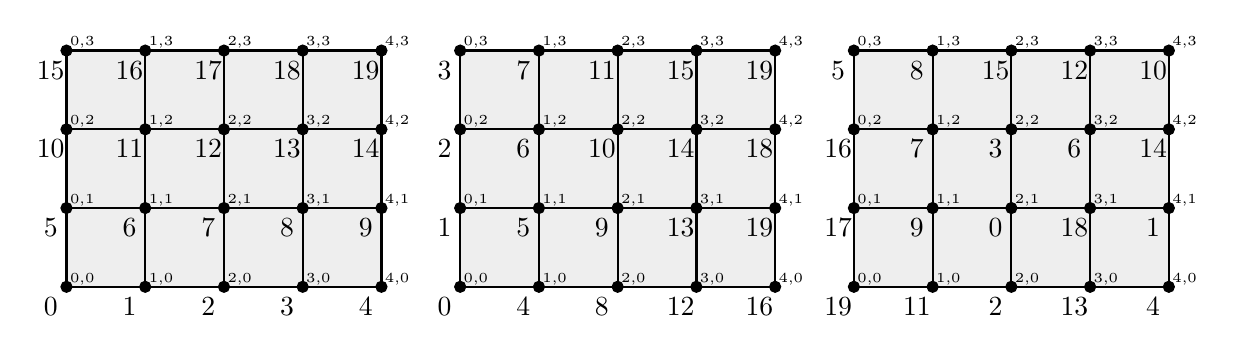
\begin{tikzpicture}
%\draw[fill=gray!23,gray!23](0,0) rectangle (17,5);
%\draw[step=0.5cm,gray,very thin] (0,0) grid (17,5); %background grid

\draw[fill=gray!13,gray!13](1,1) rectangle (5,4);
\draw[fill=gray!13,gray!13](6,1) rectangle (10,4);
\draw[fill=gray!13,gray!13](11,1) rectangle (15,4);

\draw[thick] (1,1) -- (5,1) -- (5,4) -- (1,4) -- cycle;  
\draw[thick] (1,2) -- (5,2) ; 
\draw[thick] (1,3) -- (5,3) ; 
\draw[thick] (2,1) -- (2,4) ; 
\draw[thick] (3,1) -- (3,4) ; 
\draw[thick] (4,1) -- (4,4) ; 
\node[] at (0.8,0.75) {0};
\node[] at (1.8,0.75) {1};
\node[] at (2.8,0.75) {2};
\node[] at (3.8,0.75) {3};
\node[] at (4.8,0.75) {4};
\node[] at (0.8,1.75) {5};
\node[] at (1.8,1.75) {6};
\node[] at (2.8,1.75) {7};
\node[] at (3.8,1.75) {8};
\node[] at (4.8,1.75) {9};
\node[] at (0.8,2.75) {10};
\node[] at (1.8,2.75) {11};
\node[] at (2.8,2.75) {12};
\node[] at (3.8,2.75) {13};
\node[] at (4.8,2.75) {14};
\node[] at (0.8,3.75) {15};
\node[] at (1.8,3.75) {16};
\node[] at (2.8,3.75) {17};
\node[] at (3.8,3.75) {18};
\node[] at (4.8,3.75) {19};
\node[] at (1.2,1.1) {\tiny{0,0}};
\node[] at (2.2,1.1) {\tiny{1,0}};
\node[] at (3.2,1.1) {\tiny{2,0}};
\node[] at (4.2,1.1) {\tiny{3,0}};
\node[] at (5.2,1.1) {\tiny{4,0}};
\node[] at (1.2,2.1) {\tiny{0,1}};
\node[] at (2.2,2.1) {\tiny{1,1}};
\node[] at (3.2,2.1) {\tiny{2,1}};
\node[] at (4.2,2.1) {\tiny{3,1}};
\node[] at (5.2,2.1) {\tiny{4,1}};
\node[] at (1.2,3.1) {\tiny{0,2}};
\node[] at (2.2,3.1) {\tiny{1,2}};
\node[] at (3.2,3.1) {\tiny{2,2}};
\node[] at (4.2,3.1) {\tiny{3,2}};
\node[] at (5.2,3.1) {\tiny{4,2}};
\node[] at (1.2,4.1) {\tiny{0,3}};
\node[] at (2.2,4.1) {\tiny{1,3}};
\node[] at (3.2,4.1) {\tiny{2,3}};
\node[] at (4.2,4.1) {\tiny{3,3}};
\node[] at (5.2,4.1) {\tiny{4,3}};
\draw[black,fill=black] (1,1)  circle (2pt);
\draw[black,fill=black] (2,1)  circle (2pt);
\draw[black,fill=black] (3,1)  circle (2pt);
\draw[black,fill=black] (4,1)  circle (2pt);
\draw[black,fill=black] (5,1)  circle (2pt);
\draw[black,fill=black] (1,2)  circle (2pt);
\draw[black,fill=black] (2,2)  circle (2pt);
\draw[black,fill=black] (3,2)  circle (2pt);
\draw[black,fill=black] (4,2)  circle (2pt);
\draw[black,fill=black] (5,2)  circle (2pt);
\draw[black,fill=black] (1,3)  circle (2pt);
\draw[black,fill=black] (2,3)  circle (2pt);
\draw[black,fill=black] (3,3)  circle (2pt);
\draw[black,fill=black] (4,3)  circle (2pt);
\draw[black,fill=black] (5,3)  circle (2pt);
\draw[black,fill=black] (1,4)  circle (2pt);
\draw[black,fill=black] (2,4)  circle (2pt);
\draw[black,fill=black] (3,4)  circle (2pt);
\draw[black,fill=black] (4,4)  circle (2pt);
\draw[black,fill=black] (5,4)  circle (2pt);
%---------------------------------------------------
\draw[thick] (6,1) -- (10,1) -- (10,4) -- (6,4) -- cycle;  
\draw[thick] (6,2) -- (10,2) ; 
\draw[thick] (6,3) -- (10,3) ; 
\draw[thick] (7,1) -- (7,4) ; 
\draw[thick] (8,1) -- (8,4) ; 
\draw[thick] (9,1) -- (9,4) ; 
\node[] at (6.2,1.1) {\tiny{0,0}};
\node[] at (7.2,1.1) {\tiny{1,0}};
\node[] at (8.2,1.1) {\tiny{2,0}};
\node[] at (9.2,1.1) {\tiny{3,0}};
\node[] at (10.2,1.1) {\tiny{4,0}};
\node[] at (6.2,2.1) {\tiny{0,1}};
\node[] at (7.2,2.1) {\tiny{1,1}};
\node[] at (8.2,2.1) {\tiny{2,1}};
\node[] at (9.2,2.1) {\tiny{3,1}};
\node[] at (10.2,2.1) {\tiny{4,1}};
\node[] at (6.2,3.1) {\tiny{0,2}};
\node[] at (7.2,3.1) {\tiny{1,2}};
\node[] at (8.2,3.1) {\tiny{2,2}};
\node[] at (9.2,3.1) {\tiny{3,2}};
\node[] at (10.2,3.1) {\tiny{4,2}};
\node[] at (6.2,4.1) {\tiny{0,3}};
\node[] at (7.2,4.1) {\tiny{1,3}};
\node[] at (8.2,4.1) {\tiny{2,3}};
\node[] at (9.2,4.1) {\tiny{3,3}};
\node[] at (10.2,4.1) {\tiny{4,3}};
\draw[black,fill=black] (6,1)  circle (2pt);
\draw[black,fill=black] (7,1)  circle (2pt);
\draw[black,fill=black] (8,1)  circle (2pt);
\draw[black,fill=black] (9,1)  circle (2pt);
\draw[black,fill=black] (10,1)  circle (2pt);
\draw[black,fill=black] (6,2)  circle (2pt);
\draw[black,fill=black] (7,2)  circle (2pt);
\draw[black,fill=black] (8,2)  circle (2pt);
\draw[black,fill=black] (9,2)  circle (2pt);
\draw[black,fill=black] (10,2)  circle (2pt);
\draw[black,fill=black] (6,3)  circle (2pt);
\draw[black,fill=black] (7,3)  circle (2pt);
\draw[black,fill=black] (8,3)  circle (2pt);
\draw[black,fill=black] (9,3)  circle (2pt);
\draw[black,fill=black] (10,3)  circle (2pt);
\draw[black,fill=black] (6,4)  circle (2pt);
\draw[black,fill=black] (7,4)  circle (2pt);
\draw[black,fill=black] (8,4)  circle (2pt);
\draw[black,fill=black] (9,4)  circle (2pt);
\draw[black,fill=black] (10,4)  circle (2pt);
\node[] at (5.8,0.75) {0};
\node[] at (6.8,0.75) {4};
\node[] at (7.8,0.75) {8};
\node[] at (8.8,0.75) {12};
\node[] at (9.8,0.75) {16};
\node[] at (5.8,1.75) {1};
\node[] at (6.8,1.75) {5};
\node[] at (7.8,1.75) {9};
\node[] at (8.8,1.75) {13};
\node[] at (9.8,1.75) {19};
\node[] at (5.8,2.75) {2};
\node[] at (6.8,2.75) {6};
\node[] at (7.8,2.75) {10};
\node[] at (8.8,2.75) {14};
\node[] at (9.8,2.75) {18};
\node[] at (5.8,3.75) {3};
\node[] at (6.8,3.75) {7};
\node[] at (7.8,3.75) {11};
\node[] at (8.8,3.75) {15};
\node[] at (9.8,3.75) {19};

%---------------------------------------------------
\draw[thick] (11,1) -- (15,1) -- (15,4) -- (11,4) -- cycle;  
\draw[thick] (11,2) -- (15,2) ; 
\draw[thick] (11,3) -- (15,3) ; 
\draw[thick] (12,1) -- (12,4) ; 
\draw[thick] (13,1) -- (13,4) ; 
\draw[thick] (14,1) -- (14,4) ; 
\node[] at (11.2,1.1) {\tiny{0,0}};
\node[] at (12.2,1.1) {\tiny{1,0}};
\node[] at (13.2,1.1) {\tiny{2,0}};
\node[] at (14.2,1.1) {\tiny{3,0}};
\node[] at (15.2,1.1) {\tiny{4,0}};
\node[] at (11.2,2.1) {\tiny{0,1}};
\node[] at (12.2,2.1) {\tiny{1,1}};
\node[] at (13.2,2.1) {\tiny{2,1}};
\node[] at (14.2,2.1) {\tiny{3,1}};
\node[] at (15.2,2.1) {\tiny{4,1}};
\node[] at (11.2,3.1) {\tiny{0,2}};
\node[] at (12.2,3.1) {\tiny{1,2}};
\node[] at (13.2,3.1) {\tiny{2,2}};
\node[] at (14.2,3.1) {\tiny{3,2}};
\node[] at (15.2,3.1) {\tiny{4,2}};
\node[] at (11.2,4.1) {\tiny{0,3}};
\node[] at (12.2,4.1) {\tiny{1,3}};
\node[] at (13.2,4.1) {\tiny{2,3}};
\node[] at (14.2,4.1) {\tiny{3,3}};
\node[] at (15.2,4.1) {\tiny{4,3}};
\draw[black,fill=black] (11,1)  circle (2pt);
\draw[black,fill=black] (12,1)  circle (2pt);
\draw[black,fill=black] (13,1)  circle (2pt);
\draw[black,fill=black] (14,1)  circle (2pt);
\draw[black,fill=black] (15,1)  circle (2pt);
\draw[black,fill=black] (11,2)  circle (2pt);
\draw[black,fill=black] (12,2)  circle (2pt);
\draw[black,fill=black] (13,2)  circle (2pt);
\draw[black,fill=black] (14,2)  circle (2pt);
\draw[black,fill=black] (15,2)  circle (2pt);
\draw[black,fill=black] (11,3)  circle (2pt);
\draw[black,fill=black] (12,3)  circle (2pt);
\draw[black,fill=black] (13,3)  circle (2pt);
\draw[black,fill=black] (14,3)  circle (2pt);
\draw[black,fill=black] (15,3)  circle (2pt);
\draw[black,fill=black] (11,4)  circle (2pt);
\draw[black,fill=black] (12,4)  circle (2pt);
\draw[black,fill=black] (13,4)  circle (2pt);
\draw[black,fill=black] (14,4)  circle (2pt);
\draw[black,fill=black] (15,4)  circle (2pt);
\node[] at (10.8,0.75) {19};
\node[] at (11.8,0.75) {11};
\node[] at (12.8,0.75) {2};
\node[] at (13.8,0.75) {13};
\node[] at (14.8,0.75) {4};
\node[] at (10.8,1.75) {17};
\node[] at (11.8,1.75) {9};
\node[] at (12.8,1.75) {0};
\node[] at (13.8,1.75) {18};
\node[] at (14.8,1.75) {1};
\node[] at (10.8,2.75) {16};
\node[] at (11.8,2.75) {7};
\node[] at (12.8,2.75) {3};
\node[] at (13.8,2.75) {6};
\node[] at (14.8,2.75) {14};
\node[] at (10.8,3.75) {5};
\node[] at (11.8,3.75) {8};
\node[] at (12.8,3.75) {15};
\node[] at (13.8,3.75) {12};
\node[] at (14.8,3.75) {10};


\end{tikzpicture}
\\
\end{minipage}
%-/-/-/-/-/-/-/-/-/-/-/-/-/-/-/

\vspace{.5cm}

This is a critical point because the discretised PDE is formulated as a function of $T_{{\color{brown} i,j}}$ 
with ${\color{brown}i}=0,\dot nnx-1$ and ${\color{brown}j}=0,\dots nny-1$ 
but the vector $\vec{T}$ containing all these values
is indexed by a single index ${\color{teal}k}=0,\dots nnp-1$. The numbering strategy determines how easy
it is to go from $({\color{brown}i},{\color{brown}j})$ to ${\color{teal}k}$ and vice versa. 
Very concretely again, where does $T_{\color{brown}3,4}$ should be placed in the global 
vector of unknowns $\vec{T}$?

We then need a (preferably simple/straightforward) 'function' 
which associates to every $({\color{brown} i,j})$ a global index $k$. 
For the first grid with row-wise numbering, we have 
$0\leq {\color{brown}i} \leq 4$ , $0 \leq {\color{brown}j} \leq 3$ 
so that $0 \leq {\color{teal}k} \leq 19$
and it follows that 
\begin{equation}
{\color{teal} k}={\color{brown}j}*nnx+{\color{brown}i}
\end{equation}
This is easy to verify: ${\color{brown}i}=3$ and ${\color{brown}j}=2$ 
indeed corresponds to node \# 13, 
${\color{brown}i}=4$ and ${\color{brown}j}=1$ corresponds to node \# 9, etc ...

%-/-/-/-/-/-/-/-/-/-/-/-/-/-/-/
\begin{minipage}[t]{\textwidth}
\begin{center}


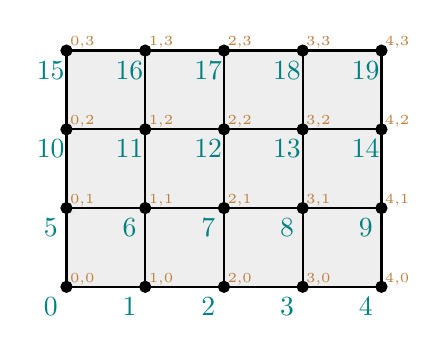
\begin{tikzpicture}
%\draw[fill=gray!23,gray!23](0,0) rectangle (8,5);
%\draw[step=0.5cm,gray,very thin] (0,0) grid (8,5); %background grid


\draw[fill=gray!13,gray!13](1,1) rectangle (5,4);
\draw[thick] (1,1) -- (5,1) -- (5,4) -- (1,4) -- cycle;  

\draw[thick] (1,2) -- (5,2) ; 
\draw[thick] (1,3) -- (5,3) ; 
\draw[thick] (2,1) -- (2,4) ; 
\draw[thick] (3,1) -- (3,4) ; 
\draw[thick] (4,1) -- (4,4) ; 

\node[] at (0.8,0.75) {\color{teal} 0};
\node[] at (1.8,0.75) {\color{teal} 1};
\node[] at (2.8,0.75) {\color{teal} 2};
\node[] at (3.8,0.75) {\color{teal} 3};
\node[] at (4.8,0.75) {\color{teal} 4};
\node[] at (0.8,1.75) {\color{teal} 5};
\node[] at (1.8,1.75) {\color{teal} 6};
\node[] at (2.8,1.75) {\color{teal} 7};
\node[] at (3.8,1.75) {\color{teal} 8};
\node[] at (4.8,1.75) {\color{teal} 9};
\node[] at (0.8,2.75) {\color{teal} 10};
\node[] at (1.8,2.75) {\color{teal} 11};
\node[] at (2.8,2.75) {\color{teal} 12};
\node[] at (3.8,2.75) {\color{teal} 13};
\node[] at (4.8,2.75) {\color{teal} 14};
\node[] at (0.8,3.75) {\color{teal} 15};
\node[] at (1.8,3.75) {\color{teal} 16};
\node[] at (2.8,3.75) {\color{teal} 17};
\node[] at (3.8,3.75) {\color{teal} 18};
\node[] at (4.8,3.75) {\color{teal} 19};

\node[] at (1.2,1.1) {\tiny{\color{brown}0,0}};
\node[] at (2.2,1.1) {\tiny{\color{brown}1,0}};
\node[] at (3.2,1.1) {\tiny{\color{brown}2,0}};
\node[] at (4.2,1.1) {\tiny{\color{brown}3,0}};
\node[] at (5.2,1.1) {\tiny{\color{brown}4,0}};
\node[] at (1.2,2.1) {\tiny{\color{brown}0,1}};
\node[] at (2.2,2.1) {\tiny{\color{brown}1,1}};
\node[] at (3.2,2.1) {\tiny{\color{brown}2,1}};
\node[] at (4.2,2.1) {\tiny{\color{brown}3,1}};
\node[] at (5.2,2.1) {\tiny{\color{brown}4,1}};
\node[] at (1.2,3.1) {\tiny{\color{brown}0,2}};
\node[] at (2.2,3.1) {\tiny{\color{brown}1,2}};
\node[] at (3.2,3.1) {\tiny{\color{brown}2,2}};
\node[] at (4.2,3.1) {\tiny{\color{brown}3,2}};
\node[] at (5.2,3.1) {\tiny{\color{brown}4,2}};
\node[] at (1.2,4.1) {\tiny{\color{brown}0,3}};
\node[] at (2.2,4.1) {\tiny{\color{brown}1,3}};
\node[] at (3.2,4.1) {\tiny{\color{brown}2,3}};
\node[] at (4.2,4.1) {\tiny{\color{brown}3,3}};
\node[] at (5.2,4.1) {\tiny{\color{brown}4,3}};

\draw[black,fill=black] (1,1)  circle (2pt);
\draw[black,fill=black] (2,1)  circle (2pt);
\draw[black,fill=black] (3,1)  circle (2pt);
\draw[black,fill=black] (4,1)  circle (2pt);
\draw[black,fill=black] (5,1)  circle (2pt);
\draw[black,fill=black] (1,2)  circle (2pt);
\draw[black,fill=black] (2,2)  circle (2pt);
\draw[black,fill=black] (3,2)  circle (2pt);
\draw[black,fill=black] (4,2)  circle (2pt);
\draw[black,fill=black] (5,2)  circle (2pt);
\draw[black,fill=black] (1,3)  circle (2pt);
\draw[black,fill=black] (2,3)  circle (2pt);
\draw[black,fill=black] (3,3)  circle (2pt);
\draw[black,fill=black] (4,3)  circle (2pt);
\draw[black,fill=black] (5,3)  circle (2pt);
\draw[black,fill=black] (1,4)  circle (2pt);
\draw[black,fill=black] (2,4)  circle (2pt);
\draw[black,fill=black] (3,4)  circle (2pt);
\draw[black,fill=black] (4,4)  circle (2pt);
\draw[black,fill=black] (5,4)  circle (2pt);

%\draw[black,fill=black] (3.1,0.2) circle (2pt); \node[] at (3.4,0.2) {$\vec\upnu$};
%\draw (4.1,0.2) circle (4pt); \node[] at (4.4,0.2) {$p$};
%\node[] at (2.5,4.5) {4 vel. nodes, 1 press. nodes};
\end{tikzpicture}

\end{center}
\end{minipage}
%-/-/-/-/-/-/-/-/-/-/-/-/-/-/-/





%.............................
\paragraph{Explicit scheme} The simplest approach is an {\color{olive} FTCS} 
(forward time, centered space) explicit method like in 1D:
\begin{equation}
\frac{T_{{\color{brown}i,j}}^{n+1}-T_{{\color{brown}i,j}}^n}{\delta t}
= \kappa
\left(
\frac{ T_{{\color{brown}i-1,j}}^{n}-2T_{{\color{brown}i,j}}^{n}+T_{{\color{brown}i+1,j}}^{n}  }{h_x^2} + 
\frac{ T_{{\color{brown}i,j-1}}^{n}-2T_{{\color{brown}i,j}}^{n}+T_{{\color{brown}i,j+1}}^{n}  }{h_y^2}
\right)
+\frac{Q_{{\color{brown}i,j}}^n}{\rho C_p}
\end{equation}
where we have assumed that the source term $Q$ can depend of space coordinates and therefore 
appears as $Q_{{\color{brown}i},{\color{brown}j}}$ in the equation.
We define $s_x$ and $s_y$ as follows:
\begin{equation}
s_x = \frac{\kappa \delta t}{h_x^2}
\quad\quad
s_y = \frac{\kappa \delta t}{h_y^2}
\end{equation}
so that
\begin{equation}
T_{{\color{brown}i,j}}^{n+1} = T_{{\color{brown}i,j}}^n 
+ s_x ( T_{{\color{brown}i-1,j}}^{n}
-2T_{{\color{brown}i,j}}^{n}
+T_{{\color{brown}i+1,j}}^{n} ) 
+s_y ( T_{{\color{brown}i,j-1}}^{n}
-2T_{{\color{brown}i,j}}^{n}
+T_{{\color{brown}i,j+1}}^{n} ) + 
\frac{Q_{{\color{brown}i,j}}^n \delta t}{\rho C_p}
\end{equation}
The scheme is stable for  
\begin{equation}
\delta t \leq \frac{\min(h_x^2,h_y^2)}{2 \kappa}
\end{equation}
Boundary conditions can be set the usual way: for example a constant (Dirichlet) temperature 
at node $({\color{brown}i},{\color{brown}j})$ is given by
\begin{equation}
T_{{\color{brown}i},{\color{brown}j}}=T_{bc} 
\end{equation}
where $T_{bc}$ is the prescribed temperature. 

%-/-/-/-/-/-/-/-/-/-/-/-/-/-/-/-/-/-/-/
\begin{center}
\begin{minipage}[t]{0.77\textwidth}
\par\noindent\rule{\textwidth}{0.4pt}
\begin{center}

\includegraphics[width=0.8cm]{images/garftr} \\
{\color{orange}Exercise 5}
\end{center}
%-/-/-/-/-/-/-/-/-/-/-/-/-/-/-/-/-/-/-/


A simple (time-dependent) analytical solution for the temperature equation exists for 
the case that the initial temperature distribution is
\begin{equation}
T(x,y,t=0) = T_{max} \exp \left[ -\frac{x^2+y^2}{\sigma^2}   \right]
\end{equation}
where $T_{max}$ is the maximum amplitude of the temperature perturbation 
at $(x,y) = (0, 0)$ and $\sigma$ its half-width. The solution is
\begin{equation}
T(x,y,t)=\frac{T_{max}}{1+4t\kappa/\sigma^2 } \exp \left[ -\frac{x^2+y^2}{\sigma^2 + 4t\kappa}   \right]
\end{equation}
Program the analytical solution and compare it with the explicit 
numerical solution with the same initial conditions at each time step. 
Comment on the accuracy of both methods for different values of dt.

REVISIT AFTER notebook is built.

%The domain is $L_x \times L_y = 10\times 5$km. 
%Its initial temperature is $T=111\degree$C for $y<x$
%and $T=222\degree$C otherwise.
%Boundary conditions $T=150$ are prescribed on all four sides.
%Physical parameters are $\kappa=10^{-6}$.
%Compute the steady state temperature in the domain.
\par\noindent\rule{\textwidth}{0.4pt}
\end{minipage}
\end{center}



%...........................
\paragraph{Implicit scheme} 
If we now employ a fully implicit, unconditionally stable discretization scheme, the discretised 
PDE becomes:
\begin{equation}
\frac{T_{{\color{brown}i},{\color{brown}j}}^{n+1}-T_{\color{brown}i,j}^n}{\delta t}
= \kappa
\left(
\frac{ T_{{\color{brown}i-1,j}}^{n+1}-2T_{{\color{brown}i,j}}^{n+1}+T_{{\color{brown}i+1,j}}^{n+1} }{h_x^2} + 
\frac{ T_{{\color{brown}i,j-1}}^{n+1}-2T_{{\color{brown}i,j}}^{n+1}+T_{{\color{brown}i,j+1}}^{n+1} }{h_y^2}
\right)
+\frac{Q_{{\color{brown}i,j}}^n}{\rho C_p}
\end{equation}
Rearranging terms with $n+1$ on the left and terms with $n$ on the right hand side gives
\begin{equation}
-s_x\; T_{{\color{brown}i+1,j}}^{n+1}
-s_y\; T_{{\color{brown}i,j+1}}^{n+1} 
+(1+2s_x+2s_y)\; T_{{\color{brown}i,j}}^{n+1} 
-s_x\;  T_{{\color{brown}i-1,j}}^{n+1} 
-s_y\;  T_{{\color{brown}i,j-1}}^{n+1} 
=
T_{{\color{brown}i,j}}^n
+\frac{Q_{{\color{brown}i,j}}^n \delta t}{\rho C_p}
\end{equation}
which here again yields a linear system of equations written ${\bm A}\cdot {\vec T} = {\vec b}$
where ${\bm A}$ is a $(nnp \times nnp)$ matrix.

Boundary conditions are $T(x,y)=0$ on all sides, so all nodes 
on the boundary have a prescribed zero temperature\footnote{We assume
here again that these boundary conditions do not change with time.}:
\begin{eqnarray}
T_{\color{brown}0,0} = T_{\color{teal} 0} &=& 0 \nn\\
T_{\color{brown}1,0} = T_{\color{teal} 1} &=& 0 \nn\\
T_{\color{brown}2,0} = T_{\color{teal} 2} &=& 0 \nn\\
T_{\color{brown}3,0} = T_{\color{teal} 3} &=& 0 \nn\\
T_{\color{brown}4,0} = T_{\color{teal} 4} &=& 0 \nn\\
T_{\color{brown}0,1} = T_{\color{teal} 5} &=& 0 \nn\\
T_{\color{brown}4,1} = T_{\color{teal} 9} &=& 0 \nn\\
T_{\color{brown}0,2} = T_{\color{teal} 10} &=& 0 \nn\\
T_{\color{brown}4,2} = T_{\color{teal} 14} &=& 0 \nn\\
T_{\color{brown}0,3} = T_{\color{teal} 15} &=& 0 \nn\\
T_{\color{brown}1,3} = T_{\color{teal} 16} &=& 0 \nn\\
T_{\color{brown}2,3} = T_{\color{teal} 17} &=& 0 \nn\\
T_{\color{brown}3,3} = T_{\color{teal} 18} &=& 0 \nn\\
T_{\color{brown}4,3} = T_{\color{teal} 19} &=& 0 \nn
\end{eqnarray}
In what follows we assume for simplicity and conciseness of notation that 
$h_x=h_y=h$ so that $s_x=s_y=s$ and we will use the notation $\tilde{Q}=Q \delta t/\rho C_p$.
The discretised PDE equation will now be applied to the interior nodes:
\begin{eqnarray}
-s T_{{\color{brown} i+1,j}}^{n+1}
-s T_{{\color{brown}i,j+1}}^{n+1} 
+(1+4s)T_{{\color{brown}i,j}}^{n+1} 
-s T_{{\color{brown}i-1,j}}^{n+1} 
-s T_{{\color{brown}i,j-1}}^{n+1} 
= T_{{\color{brown}i,j}}^n 
+\tilde{Q}_{{\color{brown}i,j}}^n
\end{eqnarray}

\begin{itemize}
\item For node ${\color{teal}k}=6$ (${\color{brown}i}=1,{\color{brown}j}=1$):
\begin{equation}
-s T_{{\color{brown}2,1}}^{n+1}
-s T_{{\color{brown}1,2}}^{n+1} 
+(1+4s)T_{{\color{brown}1,1}}^{n+1} 
-s T_{{\color{brown}0,1}}^{n+1} 
-s T_{{\color{brown}1,0}}^{n+1} 
= T_{{\color{brown}1,1}}^n +\tilde{Q}_{{\color{brown}1,1}}^n
\end{equation}
or, 
\begin{equation}
-s T_{\color{teal} 7}^{n+1}-s T_{\color{teal} 11}^{n+1} +(1+4s)T_{\color{teal} 6}^{n+1} -s T_{\color{teal} 5}^{n+1} -s T_{\color{teal} 1}^{n+1} 
= T_{\color{teal} 6}^n +\tilde{Q}_{\color{teal} 6}^n
\end{equation}

\item For node ${\color{teal}k}=7$ (${\color{brown}i}=2,{\color{brown}j}=1$):
\begin{equation}
-s T_{{\color{brown} 3,1}}^{n+1}
-s T_{{\color{brown}2,2}}^{n+1} 
+(1+4s)T_{{\color{brown}2,1}}^{n+1} 
-s T_{{\color{brown}1,1}}^{n+1} 
-s T_{{\color{brown}2,0}}^{n+1} 
= T_{{\color{brown}2,1}}^n 
+\tilde{Q}_{{\color{brown}2,1}}^n
\end{equation}
or,


\item For node ${\color{teal}k}=8$ (${\color{brown}i}=3,{\color{brown}j}=1$):
\[
-s T_{{\color{brown} 4,1}}^{n+1}
-s T_{{\color{brown}3,2}}^{n+1} 
+(1+4s)T_{{\color{brown}3,1}}^{n+1} 
-s T_{{\color{brown}2,1}}^{n+1} 
-s T_{{\color{brown}3,0}}^{n+1} 
= T_{{\color{brown}3,1}}^n 
+\tilde{Q}_{{\color{brown}3,1}}^n
\]
or,
\item For node ${\color{teal}k}=11$ (${\color{brown}i}=1,{\color{brown}j}=2$):
\[
-s T_{{\color{brown} i+1,j}}^{n+1}
-s T_{{\color{brown}i,j+1}}^{n+1} 
+(1+4s)T_{{\color{brown}1,2}}^{n+1} 
-s T_{{\color{brown}i-1,j}}^{n+1} 
-s T_{{\color{brown}i,j-1}}^{n+1} 
= T_{{\color{brown}1,2}}^n 
+\tilde{Q}_{{\color{brown}1,2}}^n
\]
or,
\item For node ${\color{teal}k}=12$ (${\color{brown}i}=2,{\color{brown}j}=2$):
\[
-s T_{{\color{brown} 3,2}}^{n+1}
-s T_{{\color{brown}2,3}}^{n+1} 
+(1+4s)T_{{\color{brown}2,2}}^{n+1} 
-s T_{{\color{brown}1,2}}^{n+1} 
-s T_{{\color{brown}2,1}}^{n+1} 
= T_{{\color{brown}2,2}}^n 
+\tilde{Q}_{{\color{brown}2,2}}^n
\]
or,
\[
-s T_{{\color{teal} 13}}^{n+1}
-s T_{{\color{teal} 17}}^{n+1} 
+(1+4s)T_{{\color{teal}12}}^{n+1} 
-s T_{{\color{teal}11}}^{n+1} 
-s T_{{\color{teal}7}}^{n+1} 
= T_{{\color{teal}12}}^n 
+\tilde{Q}_{{\color{teal}12}}^n
\]


\item For node ${\color{teal}k}=13$ (${\color{brown}i}=3,{\color{brown}j}=2$):
\begin{eqnarray}
-s T_{{\color{brown} 4,2}}^{n+1}
-s T_{{\color{brown}3,3}}^{n+1} 
+(1+4s)T_{{\color{brown}3,2}}^{n+1} 
-s T_{{\color{brown}2,2}}^{n+1} 
-s T_{{\color{brown}3,1}}^{n+1} 
&=& T_{{\color{brown}3,2}}^n 
+\tilde{Q}_{{\color{brown}3,2}}^n \nn\\
\Rightarrow \qquad
-s T_{{\color{teal} 14}}^{n+1}
-s T_{{\color{teal} 18}}^{n+1} 
+(1+4s)T_{{\color{teal}13}}^{n+1} 
-s T_{{\color{teal}12}}^{n+1} 
-s T_{{\color{teal}8}}^{n+1} 
&=& T_{{\color{teal}13}}^n 
+\tilde{Q}_{{\color{teal}13}}^n \nn
\end{eqnarray}


\end{itemize}

Putting it all together yields the following linear system:

\begin{landscape}
\[
\underbrace{
\left(
\begin{array}{cccccccccccccccccccc}
1 & . & . & . & . & . & . & . & . & . & . & . & . & . & . & . & . & . & . & . \\ %#0
. & 1 & . & . & . & . & . & . & . & . & . & . & . & . & . & . & . & . & . & . \\ %#1
. & . & 1 & . & . & . & . & . & . & . & . & . & . & . & . & . & . & . & . & . \\ %#2
. & . & . & 1 & . & . & . & . & . & . & . & . & . & . & . & . & . & . & . & . \\ %#3
. & . & . & . & 1 & . & . & . & . & . & . & . & . & . & . & . & . & . & . & . \\ %#4
. & . & . & . & . & 1 & . & . & . & . & . & . & . & . & . & . & . & . & . & . \\ %#5
. & -s& . & . & . & -s& {1+4s} & -s& . & . & . & -s & . & . & . & . & . & . & . & . \\ %#6
. & . & -s& . & . & . & -s& {1+4s} & -s& . & . & . & -s & . & . & . & . & . & . & .\\ %#7
. & . & . & -s& . & . & . & -s & {1+4s} & -s & . & . & . & -s & . & . & . & . & . & . \\ %#8
. & . & . & . & . & . & . & . & . & 1 & . & . & . & . & . & . & . & . & . & . \\ %#9
. & . & . & . & . & . & . & . & . & . & 1 & . & . & . & . & . & . & . & . & . \\ %#10
. & . & . & . & . & . &-s & . & . & . & -s& {1+4s} & -s& . & . & .  & -s& . & . & .\\ %#11
. & . & . & . & . & . & . &-s & . & . & . & -s& {1+4s} & -s& . & . & .  & -s& . & .\\ %#12
. & . & . & . & . & . & . & . &-s & . & . & . & -s& {1+4s} & -s& . & . & .  & -s & .\\ %#13
. & . & . & . & . & . & . & . & . & . & . & . & . & . & 1 & . & . & . & . & . \\ %#14
. & . & . & . & . & . & . & . & . & . & . & . & . & . & . & 1 & . & . & . & . \\ %#15
. & . & . & . & . & . & . & . & . & . & . & . & . & . & . & . & 1 & . & . & . \\ %#16
. & . & . & . & . & . & . & . & . & . & . & . & . & . & . & . & . & 1 & . & . \\ %#17
. & . & . & . & . & . & . & . & . & . & . & . & . & . & . & . & . & . & 1 & . \\ %#18
. & . & . & . & . & . & . & . & . & . & . & . & . & . & . & . & . & . & . & 1    %#19
\end{array}
\right)
}_{\bm A}
\cdot
\underbrace{
\left(
\begin{array}{c}
T_{{\color{teal}0}}^{n+1} \\ 
T_{{\color{teal}1}}^{n+1} \\ 
T_{{\color{teal}2}}^{n+1} \\ 
T_{{\color{teal}3}}^{n+1} \\ 
T_{{\color{teal}4}}^{n+1} \\ 
T_{{\color{teal}5}}^{n+1} \\ 
T_{{\color{teal}6}}^{n+1} \\ 
T_{{\color{teal}7}}^{n+1} \\ 
T_{{\color{teal}8}}^{n+1} \\ 
T_{{\color{teal}9}}^{n+1} \\ 
T_{{\color{teal}10}}^{n+1} \\ 
T_{{\color{teal}11}}^{n+1} \\ 
T_{{\color{teal}12}}^{n+1} \\ 
T_{{\color{teal}13}}^{n+1} \\ 
T_{{\color{teal}14}}^{n+1} \\ 
T_{{\color{teal}15}}^{n+1} \\ 
T_{{\color{teal}16}}^{n+1} \\ 
T_{{\color{teal}17}}^{n+1} \\ 
T_{{\color{teal}18}}^{n+1} \\ 
T_{{\color{teal}19}}^{n+1} 
\end{array}
\right)
}_{\vec T}
=
\underbrace{
\left(
\begin{array}{c}
0\\ 
0\\ 
0\\ 
0\\ 
0\\ 
0\\ 
T_{{\color{teal}6}}^n + \tilde{Q}_{\color{teal}6} \\ 
T_{{\color{teal}7}}^n + \tilde{Q}_{\color{teal}7} \\ 
T_{{\color{teal}8}}^n + \tilde{Q}_{\color{teal}8} \\ 
0\\ 
0\\ 
T_{{\color{teal}11}}^n + \tilde{Q}_{\color{teal}11} \\ 
T_{{\color{teal}12}}^n + \tilde{Q}_{\color{teal}12} \\ 
T_{{\color{teal}13}}^n + \tilde{Q}_{\color{teal}13} \\ 
0\\ 
0\\ 
0\\ 
0\\ 
0\\ 
0 
\end{array}
\right)
}_{\vec b}
\]
Note that we now have five diagonals filled with non-zero entries as opposed to three
diagonals in the 1D case.
\end{landscape}

%-/-/-/-/-/-/-/-/-/-/-/-/-/-/-/-/-/-/-/-/-/-/
\begin{center}
\begin{minipage}[t]{0.77\textwidth}
\par\noindent\rule{\textwidth}{0.4pt}
\begin{center}

\includegraphics[width=0.8cm]{images/garftr} \\
{\color{orange}Exercise 6}
\end{center}

Same exercise as exercise 5, but now with implicit method.

\par\noindent\rule{\textwidth}{0.4pt}
\end{minipage}
\end{center}
%-/-/-/-/-/-/-/-/-/-/-/-/-/-/-/-/-/-/-/-/-/-/


Looking at this matrix, it is clear that this approach is sub-optimal: for such a small grid counting
20 nodes, the boundary conditions enforce the temperature on 14 of them, so that these
temperatures should/could be removed from the list of unknowns, leaving a vector 
of unknowns $\vec{T}$ of size 6 (the number of nodes which are not on the boundary).
As a consequence, we would have to solve a $6\times 6$ linear system, as opposed to a $20\times 20$ one!

In this case, we focus again on nodes 6,7,8,11,12,13.
we start from 
\begin{equation}
-s T_{{\color{teal} 7}}^{n+1}
-s T_{{\color{teal} 11}}^{n+1} 
+(1+4s)T_{{\color{teal} 6}}^{n+1} 
-s T_{{\color{teal} 5}}^{n+1} 
-s T_{{\color{teal} 1}}^{n+1} 
= T_{{\color{teal} 6}}^n 
+\tilde{Q}_{{\color{teal} 6}}^n
\end{equation}
but we know that the boundary conditions impose that $T_1=0$ and $T_5=0$ so that the equation above simplifies to:
\begin{equation}
-s T_{{\color{teal} 7}}^{n+1}
-s T_{{\color{teal} 11}}^{n+1} 
+(1+4s)T_{{\color{teal} 6}}^{n+1} 
= T_{{\color{teal} 6}}^n 
+\tilde{Q}_{{\color{teal} 6}}^n
\end{equation}

These 6 equations can finally be combined in the expected smaller linear system:
\begin{equation}
\underbrace{
\left(
\begin{array}{cccccc}
1+4s & -s & . & . & . & -s \\
-s & 1+4s & -s & . & -s & . \\
. & -s & 1+4s & . & . & -s \\ 
-s & . & -s & 1+4s & -s & . \\
. & -s & . & -s & 1+4s & -s \\
. & . & -s & . & -s & 1+4s 
\end{array}
\right)
}_{\bm A}
\cdot
\underbrace{
\left(
\begin{array}{c}
T_{{\color{teal}6}}^{n+1} \\ 
T_{{\color{teal}7}}^{n+1} \\ 
T_{{\color{teal}8}}^{n+1} \\ 
T_{{\color{teal}11}}^{n+1} \\ 
T_{{\color{teal}12}}^{n+1} \\ 
T_{{\color{teal}13}}^{n+1} 
\end{array}
\right)
}_{\vec T}
=
\underbrace{
\left(
\begin{array}{c}
T_{{\color{teal}6}}^n + \tilde{Q}_{\color{teal}6} \\ 
T_{{\color{teal}7}}^n + \tilde{Q}_{\color{teal}7} \\ 
T_{{\color{teal}8}}^n + \tilde{Q}_{\color{teal}8} \\ 
T_{{\color{teal}11}}^n + \tilde{Q}_{\color{teal}11} \\ 
T_{{\color{teal}12}}^n + \tilde{Q}_{\color{teal}12} \\ 
T_{{\color{teal}13}}^n + \tilde{Q}_{\color{teal}13} 
\end{array}
\right)
}_{\vec b}
\end{equation}
Note that is the boundary values had not been zero they would have found their way to the right hand side 
vector.

%STENCILS in 2D?

%-/-/-/-/-/-/-/-/-/-/-/-/-/-/-/-/-/-/
\begin{center}
\begin{minipage}[t]{0.77\textwidth}
\par\noindent\rule{\textwidth}{0.4pt}
\begin{center}

\includegraphics[width=0.8cm]{images/garftr} \\
{\color{orange}Exercise 7}
\end{center}

\par\noindent\rule{\textwidth}{0.4pt}
\end{minipage}
\end{center}
%-/-/-/-/-/-/-/-/-/-/-/-/-/-/-/-/-/-/



